% Simple level diagram, resized and in a figure environment.
\documentclass{article}

\usepackage{tikz}
\usepackage{verbatim}
\usetikzlibrary{arrows}

%=================== Define new command for simplicity
\newcommand{\len}{3} %length of the energy level
\newcommand{\spa}{7} %space the energy level
\newcommand{\off}{0.7} % vertical offset of energy display 
\newcommand{\scale}{0.4} % scale of the picture

\newcommand{\ket}[1]{$\left|#1\right\rangle$}
\newcommand{\jpi}[2]{#1$^{#2}$}
\newcommand{\iso}[2]{$^{#1}$#2}
%\newcommand{\lev}[2]{\draw [level](0,#1) -- (\len,#1) node[right]{#1, #2}}
%\newcommand{\levS}[3]{\draw [level](#3,#1) -- (#3+\len,#1) node[right]{#1, #2}}
%\newcommand{\thershold}[1]{\draw [color =red, level](\len,#1) -- (-1,#1) node[left]{#1}}

\newcommand{\lev}[3]{
	\draw [level](0,#1) -- (\len,#1) ;
	\draw (\len +0.1,#1) -- (\len +0.3, #1 + #3) -- (\len +0.6, #1 + #3);
	\node[right] at (\len +0.6,#1+#3) {#1, #2};
	}

\newcommand{\levS}[4]{
	\draw [level](#3,#1) -- (#3+\len,#1) ;
	\draw (#3+\len +0.1,#1) -- (#3+\len +0.3, #1 + #4) -- (#3+\len +0.6, #1 + #4);
	\node[right] at (#3+\len +0.6,#1+#4) {#1, #2};
	}
	
\newcommand{\thershold}[2]{
	\draw [color =red, level](\len,#1) -- (-1,#1) node[left]{#1};
	\node[color =black, above] at (-\len,#1) {#2};
	}

%================== beging of doc
\begin{document}
\pagenumbering{gobble} % remove page number, and reset it to 1 on next page.

%================== Place the TikZ picture in a figure environment.
\begin{figure}
\centerline{
  \resizebox{15cm}{!}{ %reside the picture
    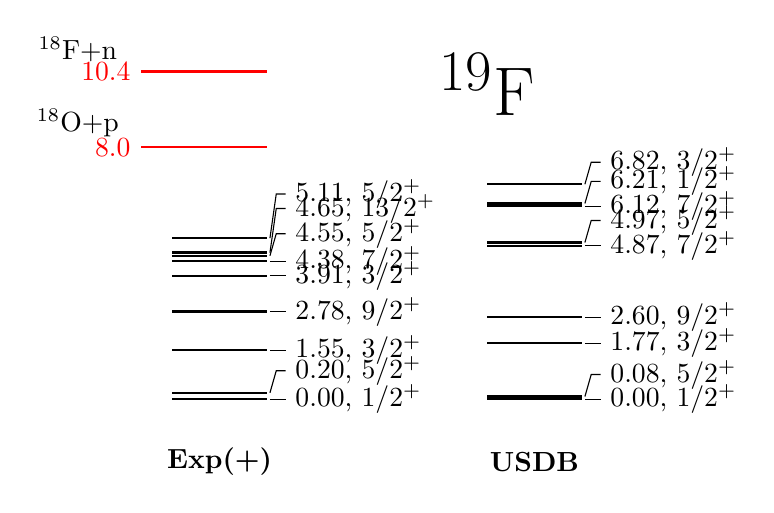
\begin{tikzpicture}[
      scale=\scale, %scale of the lines
      level/.style={thick},
      %level/.style={line width = 0.3 mm}, %another method for line width control
      virtual/.style={thick,densely dashed},
      trans/.style={thick,<->,shorten >=2pt,shorten <=2pt,>=stealth},
      classical/.style={thin,double,<->,shorten >=4pt,shorten <=4pt,>=stealth},
      label/.style = { font=\bf}
    ]
    %Name the isotope
    \node at (\len+\spa, 10){\Huge \iso{19}{F}};
    % Draw the energy levels. Exp positive parity
    \lev{0.00}{\jpi{1/2}{+}}{0};
    \lev{0.20}{\jpi{5/2}{+}}{\off};
    \lev{1.55}{\jpi{3/2}{+}}{0};
    \lev{2.78}{\jpi{9/2}{+}}{0};
    \lev{3.91}{\jpi{3/2}{+}}{0};
    \lev{4.38}{\jpi{7/2}{+}}{0};
    \lev{4.55}{\jpi{5/2}{+}}{+\off};
    \lev{4.65}{\jpi{13/2}{+}}{+2*\off};
    \lev{5.11}{\jpi{5/2}{+}}{+2*\off};
    %thershold
    \thershold{10.4}{\iso{18}{F}+n};
    \thershold{8.0}{\iso{18}{O}+p};
    %\thershold{10.6}{\iso{20}{O}+2n};
    %\thershold{18.3}{\iso{19}{O}+3n};
    % Draw another level scheme USDB
    \levS{0.00}{\jpi{1/2}{+}}{\len+\spa}{0};
    \levS{6.21}{\jpi{1/2}{+}}{\len+\spa}{+\off};
    \levS{1.77}{\jpi{3/2}{+}}{\len+\spa}{0};
    \levS{6.82}{\jpi{3/2}{+}}{\len+\spa}{+\off};
    \levS{0.08}{\jpi{5/2}{+}}{\len+\spa}{+\off};
    \levS{4.97}{\jpi{5/2}{+}}{\len+\spa}{+\off};
    \levS{4.87}{\jpi{7/2}{+}}{\len+\spa}{0};
    \levS{6.12}{\jpi{7/2}{+}}{\len+\spa}{0};
    \levS{2.60}{\jpi{9/2}{+}}{\len+\spa}{0};
    % Draw another level scheme SFO
    %\levS{0.0}{\jpi{0}{+}}{\len+\len+2*\spa}{0};
    %\levS{3.5}{\jpi{0}{+}}{\len+\len+2*\spa}{-2*\off+0.3};
    %\levS{10.5}{\jpi{0}{-}}{\len+\len+2*\spa}{+3*\off};
    %\levS{7.4}{\jpi{1}{+}}{\len+\len+2*\spa}{0};
    %\levS{9.0}{\jpi{1}{-}}{\len+\len+2*\spa}{0};
    %\levS{1.9}{\jpi{2}{+}}{\len+\len+2*\spa}{-\off};
    %\levS{3.8}{\jpi{2}{+}}{\len+\len+2*\spa}{-\off+0.4};
    %\levS{9.9}{\jpi{2}{-}}{\len+\len+2*\spa}{+2*\off};
    %\levS{4.0}{\jpi{3}{+}}{\len+\len+2*\spa}{+2*\off};
    %\levS{9.7}{\jpi{3}{-}}{\len+\len+2*\spa}{+\off/2};
    %\levS{3.8}{\jpi{4}{+}}{\len+\len+2*\spa}{+\off};
    %\levS{11.8}{\jpi{4}{-}}{\len+\len+2*\spa}{+3*\off};
    % Draw the symbol of isotopes
    \node[label] at (\len/2, -2) {Exp(+)};
    \node[label] at (\len/2+\len+\spa, -2) {USDB};
    %\node[label] at (\len/2+2*\len+2*\spa, -2) {SFO};
    \end{tikzpicture}
  }
}
\end{figure}

\end{document} 
